% BEGIN LICENSE BLOCK
% Version: CMPL 1.1
%
% The contents of this file are subject to the Cisco-style Mozilla Public
% License Version 1.1 (the "License"); you may not use this file except
% in compliance with the License.  You may obtain a copy of the License
% at www.eclipse-clp.org/license.
% 
% Software distributed under the License is distributed on an "AS IS"
% basis, WITHOUT WARRANTY OF ANY KIND, either express or implied.  See
% the License for the specific language governing rights and limitations
% under the License. 
% 
% The Original Code is  The ECLiPSe Constraint Logic Programming System. 
% The Initial Developer of the Original Code is  Cisco Systems, Inc. 
% Portions created by the Initial Developer are
% Copyright (C) 2006 Cisco Systems, Inc.  All Rights Reserved.
% 
% Contributor(s): 
% 
% END LICENSE BLOCK

\chapter{Working with real numbers and variables}
\label{chapreal}
%HEVEA\cutdef[1]{section}

\setcounter{topnumber}{1}

% - larger field/lake example

\section{Real number basics}

In general, real values cannot be represented exactly if the representation
is explicit.  As a result, they are usually approximated on computers by
floating point numbers, which have a finite precision.  This approximation
is sufficient for most purposes; however, in some situations it can lead to
significant error.  Worse, there is usually nothing to indicate that the
final result has significant error; this can lead to completely wrong
answers being accepted as correct.

One way to deal with this is to use \emph{interval arithmetic}.
    \index{interval arithmetic}%
The basic idea is that rather than using a single floating point value to
approximate the true real value, a pair of floating point bounds are used
which are guaranteed to enclose the true real value.  Each arithmetic
operation is performed on the interval represented by these bounds, and the
result rounded to ensure it encloses the true result.  The result is that
any uncertainty in the final result is made explicit: while the true real
value of the result is still not known exactly, it is guaranteed to lie
somewhere in the computed interval.

Of course, interval arithmetic is no panacea: it may be that the final
interval is too wide to be useful.  However this indicates that the problem
was probably ill-conditioned or poorly computed: if the same computation had
been performed with normal floating point numbers, the final floating point
value would probably not have been near the true real value, and there would
have been no indication that there might be a problem.

\index{bounded reals|(}
In \eclipse{}, such intervals are represented using the \emph{bounded real}
data type.

\quickref{Bounded reals}{
\begin{itemize}
\item Bounded reals are written as two floating point bounds separated 
	by a double underscore (e.g.\ \texttt{1.5__2.0}, \texttt{1.0__1.0},
	\texttt{3.1415926535897927__3.1415926535897936})
\item Other numeric types can be converted to bounded reals by giving them
	a \texttt{breal/1} wrapper, or by calling
	\bipref{breal/2}{../bips/kernel/arithmetic/breal-2.html} directly
\item Bounded reals are not usually entered directly by the user; normally
	they just occur as the results of computations
\item A bounded real represents a single real number whose value is
	known to lie somewhere between the bounds and is uncertain only
	because of the limited precision with which is has been calculated
\item An arithmetic operation is only performed using bounded reals if at
	least one of its arguments is a bounded real
\end{itemize}
}

An example of using bounded reals to safely compute the square root of 2:

\begin{quote}\begin{verbatim}
?- X is sqrt(breal(2)).
X = 1.4142135623730949__1.4142135623730954
Yes
\end{verbatim}\end{quote}

To see how using ordinary floating point numbers can lead to inaccuracy, try
dividing 1 by 10, and then adding it together 10 times.  Using floats the
result is not 1.0; using bounded reals the computed interval contains 1.0
and gives an indication of how much potential error there is:

\begin{quote}\begin{verbatim}
?- Y is float(1) / 10, X is Y + Y + Y + Y + Y + Y + Y + Y + Y + Y.
X = 0.99999999999999989
Y = 0.1
Yes
?- Y is breal(1) / 10, X is Y + Y + Y + Y + Y + Y + Y + Y + Y + Y.
X = 0.99999999999999978__1.0000000000000007
Y = 0.099999999999999992__0.1
Yes
\end{verbatim}\end{quote}


\section{Issues to be aware of when using bounded reals}

When working with bounded reals, some of the usual rules of arithmetic no
longer hold.  In particular, it is not always possible to determine whether
one bounded real is larger, smaller, or the same as another.  This is
because, if the intervals overlap, it is not possible to know the
relationship between the true values.

{\enableunderscores
An example of this can be seen in Figure~\ref{interval-compare}.  If the
true value of \texttt{X} is $\texttt{X}_1$, then depending upon whether the
true value of \texttt{Y} is (say) $\texttt{Y}_1$, $\texttt{Y}_2$ or
$\texttt{Y}_3$, we have \texttt{X > Y}, \texttt{X =:= Y} or \texttt{X < Y},
respectively.
}

\begin{figure}
\begin{center}
%\epsfbox{interval-compare.eps}
\resizebox{0.13\textwidth}{!}{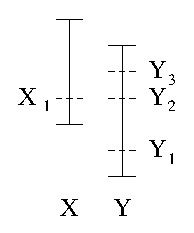
\includegraphics{interval-compare.eps}}
\end{center}
\caption{Comparing two bounded reals}
\label{interval-compare}
\end{figure}

Different classes of predicate deal with the undecidable cases in different
ways:

\index{bounded reals!comparison}

\begin{description}
\item
[Arithmetic comparison] (</2, =:=/2, etc.)
If the comparison cannot be determined definitively, the comparison succeeds
but a delayed goal is left behind, indicating that the result of the
computation is contingent on the relationship actually being true.
Examples:

\begin{quote}\begin{verbatim}
?- X = 0.2__0.3, Y = 0.0__0.1, X > Y.
X = 0.2__0.3
Y = 0.0__0.1
Yes

?- X = 0.2__0.3, Y = 0.0__0.1, X < Y.
No

?- X = 0.0__0.1, Y = 0.0__0.1, X < Y.
X = 0.0__0.1
Y = 0.0__0.1
Delayed goals:
        0.0__0.1 < 0.0__0.1
Yes

?- X = Y, X = 0.0__0.1, X < Y.
No
\end{verbatim}\end{quote}

\item
[Term equality or comparison] (=/2, ==/2, compare/3, @</2, etc.)
These predicates consider bounded reals from a purely syntactic point of
view: they determine how the bounded reals compare syntactically, without
taking into account their meaning.  Two bounded reals are considered equal
if and only if their bounds are syntactically the same (note that the
floating point numbers 0.0 and -0.0 are considered to be syntactically
different).  A unique ordering is also defined between bounded reals which
do not have identical bounds; see the documentation for compare/3 for
details.  This is important as it means predicates such as sort/2 behave in
a sensible fashion when they encounter bounded reals (in particular, they do
not throw exceptions or leave behind large numbers of meaningless delayed
goals) --- though one does need to be careful when comparing or sorting
things of different types.
Examples:

\begin{quote}\begin{verbatim}
?- X = 0.2__0.3, Y = 0.0__0.1, X == Y.
No

?- X = 0.0__0.1, Y = 0.0__0.1, X == Y.
X = 0.0__0.1
Y = 0.0__0.1
Yes

?- X = 0.2__0.3, Y = 0.0__0.1, compare(R, X, Y).
R = >
X = 0.2__0.3
Y = 0.0__0.1
Yes

?- X = 0.1__3.0, Y = 0.2__0.3, compare(R, X, Y).
R = <
X = 0.1__3.0
Y = 0.2__0.3
Yes

?- X = 0.0__0.1, Y = 0.0__0.1, compare(R, X, Y).
R = =
X = 0.0__0.1
Y = 0.0__0.1
Yes

?- sort([-5.0, 1.0__1.0], Sorted).
Sorted = [1.0__1.0, -5.0]       % 1.0__1.0 > -5.0, but 1.0__1.0 @< -5.0
Yes
\end{verbatim}\end{quote}

\end{description}

Note that the potential undecidability of arithmetic comparisons has
implications when writing general code.  For example, a common thing to do
is test the value of a number, with different code being executed depending
on whether or not it is above a certain threshold; e.g.\

\begin{code}
( X >= 0 ->
    % Code A
;
    % Code B
)
\end{code}

When writing code such as the above, if \texttt{X} could be a bounded real,
one ought to decide what should happen if \texttt{X}'s bounds span the
threshold value.  In the above example, if \texttt{X = -0.1__0.1} then a
delayed goal \texttt{-0.1__0.1 >= 0} will be left behind and Code A
executed.  If one does not want the delayed goal, one can instead write:

\begin{code}
( not X >= 0 ->
    % Code B
;
    % Code A
)
\end{code}

The use of \texttt{not} ensures that any actions performed during the test
(in particular the set up of any delayed goals) are backtracked, regardless
of the outcome of the test.

Finally, if one wishes Code B to be executed instead of Code A in the case
of an overlap, one can reverse the sense of the test:

\begin{code}
( not X < 0 ->
    % Code A
;
    % Code B
)
\end{code}

\index{bounded reals|)}


\section{IC as a solver for real variables}

\index{library!ic|(}

The IC solver is a hybrid solver which supports both real and integer
variables.

\See{See Chapter~\ref{chapicintro} for an introduction to IC and how to use
it with integer variables.}

\See{See the IC chapter in the Constraint Library Manual for a full list of
the arithmetic operators which are available for use in IC constraint
expressions.}


\quickref{Real variables and constraints}{
\begin{itemize}
\item Real variables may be declared using
	\biptxtrefni{reals/1}{reals/1!ic}{../bips/lib/ic/reals-1.html},
	\biptxtrefni{\$::/2}{\$::/2!ic}{../bips/lib/ic/SNN-2.html},
	\biptxtrefni{::/2}{::/2!ic}{../bips/lib/ic/NN-2.html} 
        \index{reals/1@\texttt{reals/1}!ic}\index{::/2@\texttt{::/2}!ic}
        \index{\$::/2@\texttt{\$::/2}!ic}(specifying
	non-integer bounds) or just by using them in an IC constraint
\item Basic constraints available for real variables are
	\biptxtrefni{\$=/2}{\$=/2!ic}{../bips/lib/ic/SE-2.html},
	\biptxtrefni{\$>=/2}{\$>=/2!ic}{../bips/lib/ic/SGE-2.html},
	\biptxtrefni{\$=</2}{\$=</2!ic}{../bips/lib/ic/SEL-2.html},
	\biptxtrefni{\$>/2}{\$>/2!ic}{../bips/lib/ic/SG-2.html},
	\biptxtrefni{\$</2}{\$</2!ic}{../bips/lib/ic/SL-2.html}
        \index{\$=/2@\texttt{\$>=/2}!ic}\index{\$=/2@\texttt{\$>=/2}!ic}
        \index{\$=</2@\texttt{\$=</2}!ic}\index{\$>/2@\texttt{\$>/2}!ic} 
        \index{\$</2@\texttt{\$</2}!ic}and
	%\biptxtrefni{\$\bsl=/2}{\$\=/2@\$$\backslash$=/2!ic}{../bips/lib/ic/ERE-2.html},
	%\biptxtrefni{\$\bsl=/2}{\$\=/2@\$\verb+\+=/2!ic}{../bips/lib/ic/ERE-2.html},
	{\bf \$\bsl=/2}
        %\html{\htmladdnormallink{\$\bsl=/2}{../bips/lib/ic/SRE-2.html}},
	%\protect\index{\$=@\$\verb+\+=/2!ic}%
	%\protect\index{\$\=@=\bsl=/2!ic}%
	as well as their reified versions and the reified connectives
\item Real constraints also work with integer variables and a mix of integer
	and real variables
\item Solutions to real constraints can be found using
	\bipref{locate/2}{../bips/lib/ic/locate-2.html},
	\bipref{locate/3}{../bips/lib/ic/locate-3.html},
	\bipref{locate/4}{../bips/lib/ic/locate-4.html} or
	\bipref{squash/3}{../bips/lib/ic/squash-3.html}
\end{itemize}
}
% This belongs inside the quickref, but the \bsl gets garbled in the index
% if it's there.
\index{\$\=@\$\bsl=/2!ic}%

IC's real constraints perform bounds propagation in the same way as the
integer versions; indeed, most of the basic integer constraints are
transformed into their real counterparts, plus a declaration of the
integrality of the variables appearing in the constraint.

Note that the interval reasoning performed to propagate real bounds is the
same as that used for bounded reals; that is, the inferences made are safe,
taking into account potential floating point errors.


\section{Finding solutions of real constraints}

In very simple cases, just imposing the constraints may be sufficient to
directly compute the (unique) solution.  For example:

\begin{quote}\begin{verbatim}
?- 3 * X $= 4.
X = 1.3333333333333333__1.3333333333333335
Yes
\end{verbatim}\end{quote}

Other times, propagation will reduce the domains of the variables to
suitably small intervals:

\begin{quote}\begin{verbatim}
?- 3 * X + 2 * Y $= 4, X - 5 * Y $= 2, X $>= -100.
Y = Y{-0.11764705946382902 .. -0.1176470540212896}
X = X{1.4117647026808551 .. 1.4117647063092196}
There are 2 delayed goals.
Yes
\end{verbatim}\end{quote}

In general though, some extra work will be needed to find the solutions of a
problem.  The IC library provides two methods for assisting with this.
Which method is appropriate depends on the nature of the solutions to be
found.  If it is expected that there a finite number of discrete solutions,
\bipref{locate/2}{../bips/lib/ic/locate-2.html} and
\bipref{locate/3}{../bips/lib/ic/locate-3.html} would be good choices.  If
solutions are expected to lie in a continuous region,
\bipref{squash/3}{../bips/lib/ic/squash-3.html} may be more appropriate.

Locate works by nondeterministically splitting the domains of the variables
until they are narrower than a specified precision (in either absolute or
relative terms).  Consider the problem of finding the points where two
circles intersect (see Figure~\ref{locatefig}).  Normal propagation does not
deduce more than the obvious bounds on the variables:

\begin{figure}
\begin{center}
%\epsfbox{locate2.eps}
\resizebox{0.13\textwidth}{!}{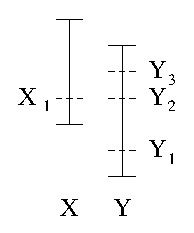
\includegraphics{interval-compare.eps}}
\end{center}
\caption{Example of using locate/2}
\label{locatefig}
\end{figure}

\begin{quote}\begin{verbatim}
?- 4 $= X^2 + Y^2, 4 $= (X - 1)^2 + (Y - 1)^2.
X = X{-1.0000000000000004 .. 2.0000000000000004}
Y = Y{-1.0000000000000004 .. 2.0000000000000004}
There are 12 delayed goals.
Yes
\end{verbatim}\end{quote}

Calling \bipref{locate/2}{../bips/lib/ic/locate-2.html} quickly determines
that there are two solutions and finds them to the desired accuracy:

\begin{quote}\begin{verbatim}
?- 4 $= X^2 + Y^2, 4 $= (X-1)^2 + (Y-1)^2, locate([X, Y], 1e-5).
X = X{-0.8228756603552696 .. -0.82287564484820042}
Y = Y{1.8228756448482002 .. 1.8228756603552694}
There are 12 delayed goals.
More

X = X{1.8228756448482004 .. 1.8228756603552696}
Y = Y{-0.82287566035526938 .. -0.82287564484820019}
There are 12 delayed goals.
Yes
\end{verbatim}\end{quote}

Squash works by deterministically cutting off parts of the domains of
variables which it determines cannot contain any solutions.  In effect, it
is like a stronger version of bounds propagation.  Consider the problem of
finding the intersection of two circular discs and a hyperplane (see
Figure~\ref{squashfig}).  Again, normal propagation does not deduce more
than the obvious bounds on the variables:

\begin{figure}
\begin{center}
%\epsfbox{squash2.eps}
\resizebox{0.47\textwidth}{!}{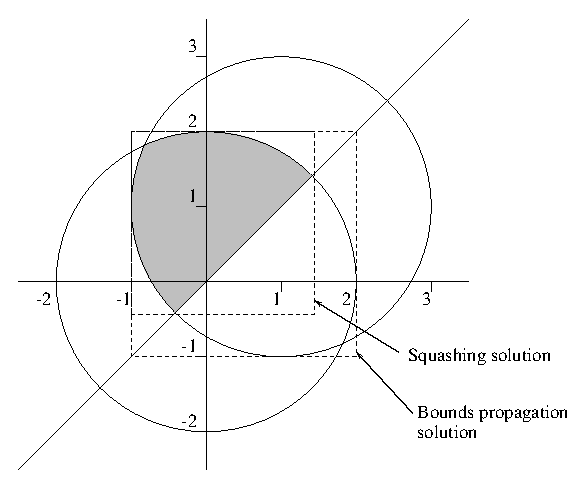
\includegraphics{squash2.eps}}
\end{center}
\caption{Example of propagation using the squash algorithm}
\label{squashfig}
\end{figure}

\begin{quote}\begin{verbatim}
?- 4 $>= X^2 + Y^2, 4 $>= (X-1)^2 + (Y-1)^2, Y $>= X.
Y = Y{-1.0000000000000004 .. 2.0000000000000004}
X = X{-1.0000000000000004 .. 2.0000000000000004}
There are 13 delayed goals.
Yes
\end{verbatim}\end{quote}

Calling \bipref{squash/3}{../bips/lib/ic/squash-3.html} results in the
bounds being tightened (in this case the bounds are tight for the feasible
region, though this is not true in general):

\begin{quote}\begin{verbatim}
?- 4 $>= X^2 + Y^2, 4 $>= (X-1)^2 + (Y-1)^2, Y $>= X,
   squash([X, Y], 1e-5, lin).
X = X{-1.0000000000000004 .. 1.4142135999632601}
Y = Y{-0.41421359996326 .. 2.0000000000000004}
There are 13 delayed goals.
Yes
\end{verbatim}\end{quote}

\See{For more details, see the IC chapter of the Library Manual or the
documentation for the individual predicates.}


\section{A larger example}
\label{farm-example}

Consider the following problem:

\begin{quote}
George is contemplating buying a farm which is a very strange shape,
comprising a large triangular lake with a square field on each side.  The
area of the lake is exactly seven acres, and the area of each field is an
exact whole number of acres.  Given that information, what is the smallest
possible total area of the three fields?
\end{quote}

A diagram of the farm is shown in Figure~\ref{lake-fields}.

\begin{figure}
\begin{center}
%\epsfbox{lake-fields.eps}
\resizebox{0.37\textwidth}{!}{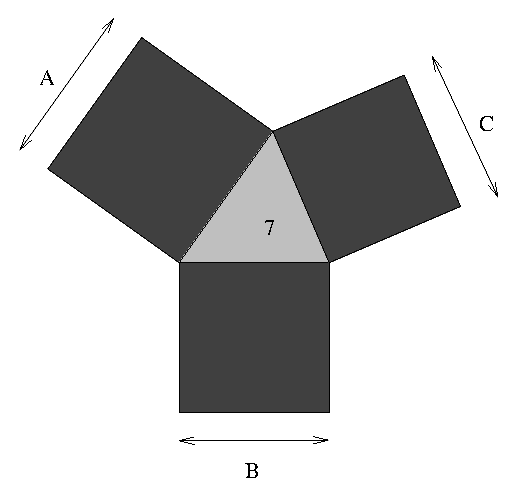
\includegraphics{lake-fields.eps}}
\end{center}
\caption{Triangular lake with adjoining square fields}
\label{lake-fields}
\end{figure}

This is a problem which mixes both integer and real quantities, and as such
is ideal for solving with the IC library.  A model for the problem appears
below.  The \texttt{farm/4} predicate sets up the constraints between the
total area of the farm \texttt{F} and the lengths of the three sides of the
lake, \texttt{A}, \texttt{B} and \texttt{C}.

\begin{code}
:- lib(ic).

farm(F, A, B, C) :-
        [A, B, C] :: 0.0 .. 1.0Inf,     % The 3 sides of the lake
        triangle_area(A, B, C, 7),      % The lake area is 7

        [F, FA, FB, FC] :: 1 .. 1.0Inf, % The square areas are integral
        square_area(A, FA),
        square_area(B, FB),
        square_area(C, FC),
        F #= FA+FB+FC,

        FA $>= FB, FB $>= FC.           % Avoid symmetric solutions

triangle_area(A, B, C, Area) :-
        S $>= 0,
        S $= (A+B+C)/2,
        Area $= sqrt(S*(S-A)*(S-B)*(S-C)).

square_area(A, Area) :-
        Area $= sqr(A).
\end{code}

A solution to the problem can then be found by first instantiating the area
of the farm, and then using \bipref{locate/2}{../bips/lib/ic/locate-2.html}
to find the lengths of the sides of the lakes.  Instantiating the area of
the farm first ensures that the first solution returned will be the minimal
one, since \bipref{indomain/1}{../bips/lib/ic/indomain-1.html} always
chooses the smallest possible value first:

\begin{code}
solve(F) :-
        farm(F, A, B, C),               % the model
        indomain(F),                    % ensure that solution is minimal
        locate([A, B, C], 0.01).
\end{code}

\section{Exercise}

\begin{enumerate}

\item

Consider the ``farm'' problem in section~\ref{farm-example}.  (Source code
may be found in \texttt{farm.ecl}, if you have access to it.) Try running
this program to find the answer.  Note that other, larger solutions are
available by selecting \emph{more}.

This implementation sums three integer variables (\texttt{FA}, \texttt{FB}
and \texttt{FC}), and then constrains their order to remove symmetries.
Would this be a good candidate for the global constraint
\texttt{ordered_sum/2}?  Modify the program so that it does use
\texttt{ordered_sum/2}.  How does the run time compare with the original?

\end{enumerate}

\index{library!ic|)}

%HEVEA\cutend
